\documentclass[landscape]{article}
\usepackage[margin=0.5in]{geometry}
\usepackage{tikz,multicol,enumitem}

\begin{document}
\thispagestyle{empty}

\newcommand{\ptable}{
  \begin{center}

    \vspace{3em}
    \noindent
    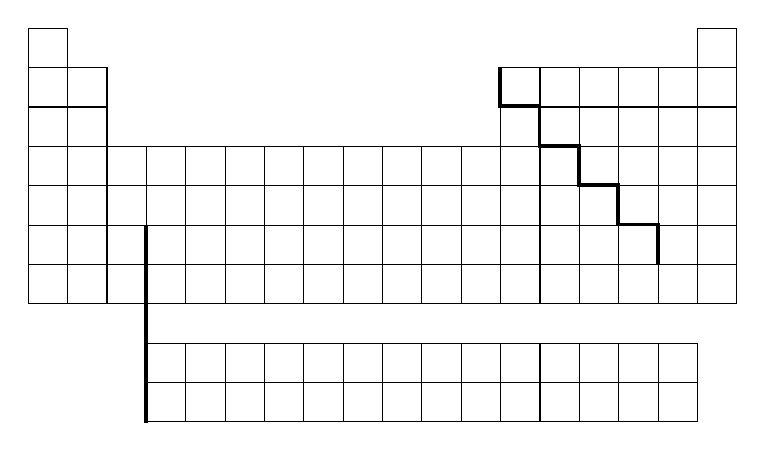
\begin{tikzpicture}
      \def\elsize{0.5cm}
      \tikzstyle{e} = [
        minimum width=\elsize, 
        minimum height=\elsize, 
        node distance=\elsize,
        draw=black
      ]
  
      \node[e, anchor=north west] at (0,0) (1) {};
  
      \node[e,below of=1] (1) {};
      \node[e,right of=1] (2) {};
  
      \node[e,below of=1] (1) {};
      \node[e,right of=1] (2) {};
  
      \node[e,below of=1] (1) {};
      \foreach \x in {1,...,17} {
        \pgfmathtruncatemacro{\y}{\x+1}
        \node[e, right of=\x] (\y) {};
      }
  
      \node[e, above of=13] (13) {};
      \foreach \x in {13,...,17} {
        \pgfmathtruncatemacro{\y}{\x+1}
        \node[e, right of=\x] (\y) {};
      }
  
      \node[e, above of=13] (13) {};
      \foreach \x in {13,...,17} {
        \pgfmathtruncatemacro{\y}{\x+1}
        \node[e, right of=\x] (\y) {};
      }
  
      \node[e, above of=18] (18) {};
  
      \foreach \per in {4,5,6} {
        \node[e, below of=1] (1) {};
        \foreach \x in {1,...,17} {
          \pgfmathtruncatemacro{\y}{\x+1}
          \node[e, right of=\x] (\y) {};
        }
      }
  
      \node[e, below of=4,node distance=2*\elsize] (4) {};
      \foreach \x in {4,...,16} {
        \pgfmathtruncatemacro{\y}{\x+1}
        \node[e, right of=\x] (\y) {};
      }
      \node[e, below of=4] (4) {};
      \foreach \x in {4,...,16} {
        \pgfmathtruncatemacro{\y}{\x+1}
        \node[e, right of=\x] (\y) {};
      }
  
      \draw[line width=.5mm] (12*\elsize,-\elsize) 
        -- ++(0,-\elsize)
        -- ++(\elsize,0)
        -- ++(0,-\elsize)
        -- ++(\elsize,0)
        -- ++(0,-\elsize)
        -- ++(\elsize,0)
        -- ++(0,-\elsize)
        -- ++(\elsize,0)
        -- ++(0,-\elsize);


      \draw[line width=0.5mm] (3*\elsize,-5*\elsize) 
        -- ++(0,-5*\elsize)
        -- ++(0,-0.15mm);
      
    \end{tikzpicture}
  \end{center}
}

\begin{multicols*}{2}
  
\section*{Valence Electrons}

\ptable

\vspace{\stretch{1}}

\section*{Ion Charges}

\ptable

\columnbreak

\section*{Valence Electrons}

\ptable

\vspace{\stretch{1}}

\section*{Ion Charges}

\ptable






\end{multicols*}


\end{document}